\documentclass{standalone}
\usepackage{tikz}
\begin{document}
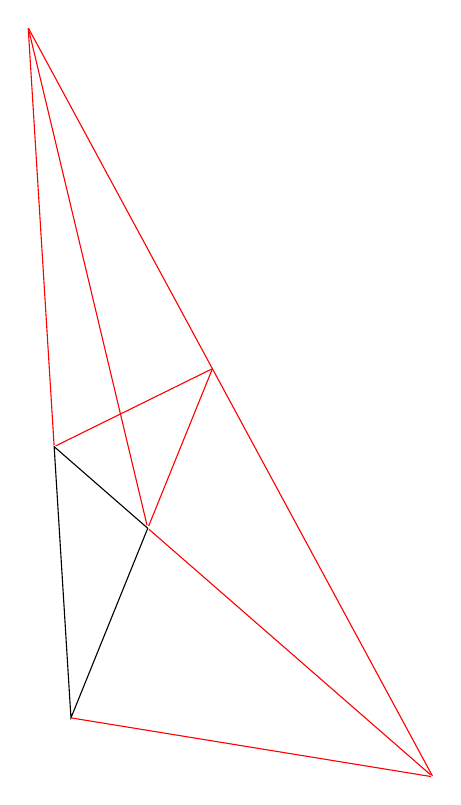
\begin{tikzpicture}[x=1pt,y=1pt]
\draw[red] (66.45,-196.29) -- (168.18,-284.97);
\draw[red] (32.12,-165.72) -- (22.79,-15.20);
\draw[red] (66.32,-195.06) -- (89.26,-138.45);
\draw[red] (65.71,-194.76) -- (23.12,-16.42);
\draw[red] (38.49,-264.44) -- (168.28,-285.59);
\draw[red] (32.66,-166.15) -- (89.19,-138.30);
\draw[red] (168.86,-285.42) -- (22.88,-15.20);
\draw (38.23,-264.41) -- (65.98,-195.89) -- (32.16,-166.40) -- cycle;
\end{tikzpicture}
\end{document}
